% The two 1-cocycles "dx" and "dy" on a torus (drawn as a square with opposite
% edges identified), each assigning values to transverse arcs.
% Source: book/tex/homology/cup-product.tex (§ de Rham cohomology, torus example).
\documentclass[border=2mm]{standalone}
\usepackage{tikz}
\usepackage{amsmath}
\usetikzlibrary{arrows.meta}
\begin{document}
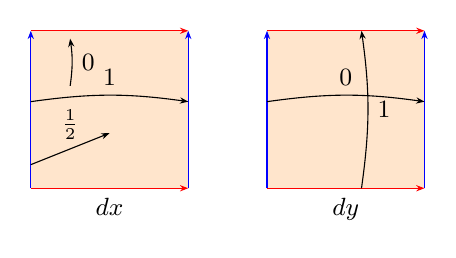
\begin{tikzpicture}[scale=1, >={Stealth[length=3pt]}, every node/.style={font=\small}]
  % left square: dx
  \fill[orange!20] (0,0) rectangle (2,2);
  \draw[blue, ->] (0,0) -- (0,2);   \draw[blue, ->] (2,0) -- (2,2);
  \draw[red, ->] (0,0) -- (2,0) node[midway, below, black] {$dx$};
  \draw[red, ->] (0,2) -- (2,2);
  \draw[->] (0,0.3) -- (1,0.7) node[midway, above] {$\tfrac12$};
  \draw[->] (0,1.1) to[bend left=8] node[midway, above] {$1$} (2,1.1);
  \draw[->] (0.5,1.3) to[bend right=8] node[midway, right] {$0$} (0.5,1.9);
  % right square: dy
  \fill[orange!20] (3,0) rectangle (5,2);
  \draw[blue, ->] (3,0) -- (3,2);   \draw[blue, ->] (5,0) -- (5,2);
  \draw[red, ->] (3,0) -- (5,0) node[midway, below, black] {$dy$};
  \draw[red, ->] (3,2) -- (5,2);
  \draw[->] (3,1.1) to[bend left=8] node[midway, above] {$0$} (5,1.1);
  \draw[->] (4.2,0) to[bend right=8] node[midway, right] {$1$} (4.2,2);
\end{tikzpicture}
\end{document}
